%%%\scalebox{1.2}{ 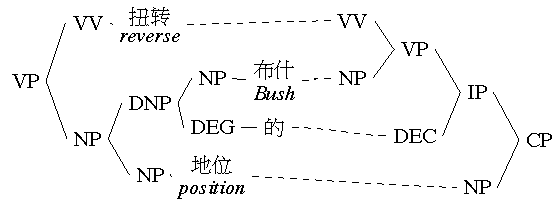
\includegraphics{figures/chinese-treebush} }

\begin{tikzpicture}
\tikzset{every tree node/.style={align=center}}
\Tree
[.\extranode{CP}
  [.\extranode{IP}
    [.\extranode{VP}
      [.VV 扭转\\reverse ]
      [.NP 布什\\Bush ] ]
    [.\extranode{DEC} 的 ] ]
  [.NP 地位\\position ] ]
\end{tikzpicture}

\vspace{3mm}
(a) Parser output

\vspace{6mm}

\begin{tikzpicture}
\tikzset{every tree node/.style={align=center}}
\Tree
[.\missingnode{VP}
  [.VV 扭转\\reverse ]
  [.\missingnode{NP}
    [.\missingnode{DNP}
      [.NP 布什\\Bush ]
      [.\missingnode{DEG} 的 ] ]
    [.NP 地位\\position ] ] ]
\end{tikzpicture}

\vspace{3mm}
(b) Gold parse
\derivspace

\caption[Error analysis example: Verb taking wrong arguments (Chinese).]{ \label{fig:wrong_arg}
  \textbf{Verb Taking Wrong Arguments} The verb takes the argument \glos{布什}{Bush} too early, before it has been bound with \glos{地位}{position}.
}
